\chapter{Wprowadzenie}
\label{cha:wstep}

Wobec mnogości i różnorodności dostępnych obecnie języków programowania, zaskoczeniem może się wydać, że istnieją pewne koncepcje językowe nigdy nie zrealizowane, bądź historycznie wypróbowane, a dziś nieobecne. W niniejszej pracy rozwinięty zostanie nowy proceduralny język programowania, wykorzystujący i łączący kilka interesujących form lingwistycznych.
Urzeczywistni się ten język poprzez program jego automatycznego translatora dla maszyn cyfrowych. Możliwość i poziom trudności skonstruowania praktycznie użytecznego kompilatora nowego języka, dysponując ograniczonymi zasobami, lecz korzystając ze współczesnych narzędzi w sposób poparty ugruntowanymi osiągnięciami lingwistyki formalnej, będzie również kluczowym przedmiotem badań.

%---------------------------------------------------------------------------

\section{Czy nowe języki programowania są potrzebne?}
\label{czy_potrzebne}
Języki ,,wysokiego poziomu'', które dziś odpowiadają powszechnemu pojęciu o ,,językach programowania'' pojawiły się w latach pięćdziesiątych ubiegłego wieku\cite[s.~13]{DRAGON_BOOK}. Wydawać by się mogło, że od tego czasu, problem, na jaki stanowiły odpowiedź - zapewnienie zrozumiałego zarówno dla człowieka jak i maszyny opisu algorytmu, po tylu dekadach doczekał się zadowalających rozwiązań - innymi słowy zaproponowano i przetestowano większość wartych uwagi możliwości i dostępne obecnie języki programowania są co najmniej wystarczające i pole do usprawnień pozostaje niewielkie.

Zdaje się mieć to odzwierciedlenie w spadającej w ostatnich latach liczbie języków nowych - takich, które zyskały publiczne uznanie i grono użytkowników\cite{valverde2015}. Powodem może być pewna dojrzałość wypracowana przez najpopularniejsze obecnie języki oraz osiągnięcie przez nie takiego poziomu abstrakcji, na którym problemy niegdyś modelowane przez specjalnie określone struktury syntaktyczne, oddać można za pomocą istniejącej, dużo ogólniejszej składni.

Przykładem niech będzie obsługa dostępu do plików w języku PL/I popularnym w latach 70, gdzie istniał dedykowany aparat składniowy, zawierający np. osobne słowo kluczowe FILE\cite[s.~96]{plif}. We współczesnym C++ czy Javie, w specyfikacji języka próżno szukać przeznaczonych do tego konstrukcji. Operacje na plikach realizowane są poprzez funkcjonalności bibliotek standardowych i nie wymagają modyfikacji języka.

Wydawać by się mogło, że po osiągnięciu pewnego poziomu abstrakcji syntaktycznej (w szczególności typów parametryzowanych), innowacje mogą ograniczyć się do rozszerzania leksykonu języka, nie modyfikując składni. Poniższy przykład, wzięty z bardzo obecnie rozpowszechnionej praktyki programistycznej ma za zadanie podważyć to twierdzenie i zwrócić uwagę na złożoność relacji pomiędzy składnią a leksykonem języka.

Napisana w Javie biblioteka Spring nie jest pierwszym i z pewnością nie ostatnim podejściem do stworzenia ekosystemu ułatwiającego rozwijanie serwerów i złożonych aplikacji sieciowych. Najtrafniejszym jej określeniem pozostanie jednak ,,framework'', ponieważ nie stanowi ona jedynie zbioru procedur gotowych do użycia, jak biblioteka, a określa również szkielet aplikacji i do pewnego stopnia redefiniuje sposób pisania programu, teoretycznie wciąż w języku Java. Niech zademonstruje to poniższy wycinek:
\begin{lstlisting}[language=java]
@Auth
@RestController
public class CarResource{
    @Autowired private CarService service;

    @Permission(Perm.CarR)
    @GetMapping("/cars")
    GetCarsResponse getCars(GetCarRequest request){
        return service.availableCars(getFilters(request));
    }
    ...
    @Permission(Perm.CarRW)
    @PostMapping("/cars")
    ReserveCarResponse reserveCar(String){...}
}
\end{lstlisting}
%spr - Spring vs Java EE
Pierwszą obserwacją niech będzie, że człowiek zaznajomiony jedynie ze specyfikacją języka Java marne ma szanse zrozumienia powyższego wycinka programu. Jeśli orientuje się w zagadnieniach sieciowych, zna pojęcie REST API i programowanie zorientowane obiektowo, może zrozumieć już bardzo wiele, potencjalnie cały zamysł programu, umknąć mu jednak mogą kluczowe szczegóły. Na przykład, zakładając, że reserveCar dokonuje modyfikacji w bazie danych, ów programista mógłby zacząć zadawać pytania o zachowanie systemu w wypadku błędu wewnątrz procedury rezerwującej samochód. Jeśli nie jest przeszkolonym użytkownikiem Springa, nie ma sposobu aby domyślił się, że pewna adnotacja nad klasą CarService, której metodę się wywołuje, odpowiada za „opakowanie” jej nową transakcją baozodanową (jeśli takowej wcześniej nie rozpoczęto) i odwinięcie jej w wypadku wystąpienia wyjątku podczas wykonania kodu wewnątrz, a jest to szczegół o potencjalnie kluczowym znaczeniu dla analizy programu.

Do jakiego stopnia jest zatem ów program napisany w Javie, do jakiego stopnia w Springu? Czy Spring jest jeszcze biblioteką, frameworkiem, czy może raczej osobnym językiem? Fakt, że ów język pozostaje podzbiorem Javy i jest wciąż tłumaczony przez jej kompilator ma jednak swoją cenę. 

Java jest w założeniach językiem kompilowanym i statycznie typowanym. Zapewniać ma to bezpieczeństwo typów, wymuszane podczas tłumaczenia programu. Poniższa linia:
\begin{lstlisting}
    CarService service = new CarService(carRepository);
\end{lstlisting}
gdy zostanie pomyślnie skompilowana, nie powinna pozostawiać pola dla wielu niespodzianek podczas wykonania.
Jeśli programista zapomni dopisać klasę CarSevice, bądź ją zaimportować aby była widoczna w tym pliku (jednostce translacji), od razu otrzyma błąd kompilacji.
Konstrukcja springowa będąca jej odpowiednikiem:
\begin{lstlisting}
@Autowired private CarService service;
\end{lstlisting}
nie zapewnia nawet tych prostych gwarancji. W podstawowym przypadku, gdy CarService fizycznie nie istnieje, faktycznie, tak samo nazwa nie zostanie odnaleziona w zakresie. Gdyby jednak wstrzykiwany obiekt był interfejsem np.,
\begin{lstlisting}
@Autowired ICarService service; 
(w innym miejscu:)CarService implements ICarService
\end{lstlisting}
albo typem parametryzowanym (w nomenklaturze Javy - generycznym)
\begin{lstlisting}
@Autowired PageableService<Car> service; 
(w innym miejscu: )CarService extends PageableService<Car>,
\end{lstlisting}
program mógłby się skompilować i dopiero przy jego uruchomieniu wystąpiłby błąd - maszyneria Springa mogłaby nie móc odnaleźć (np. z powodu błędnej konfiguracji) odpowiedniej klasy będącej podtypem interfejsu lub typu parametryzowanego. Dodatkowo, w każdym z tych trzech przypadków, włączając najprostszy, z bezpośrednim odniesieniem do nazwy klasy, Spring zawiedzie podczas wykonania, jeśli mechanizm refleksji nie będzie w stanie odnaleźć odpowiedniego konstruktora w klasie, mimo że jego istnienie lub brak, da się określić jeszcze podczas kompilacji.

Język Springa przestaje być zatem statycznie typowany, traci gwarancję sprawdzenia typów podczas przekładu. Dzieje się tak dlatego, że Spring przy całej swej złożoności pozostaje na technicznym poziomie biblioteką. Nie jest w stanie wprowadzić własnych ograniczeń do sprawdzania typów podczas kompilacji, ponieważ jego procedury same są częścią tłumaczonego programu. 

Przykład ten nie ma na celu krytyki niczego, w końcu istnieje wiele języków dynamicznie typowanych, niektóre bardzo popularne (np. Python), pokazuje,  że języki programowania, powstają zupełnie organicznie również obecnie i to w wielkich ilościach, nie nosząc wszak nazwy „języków” - wystarczy zacząć liczyć frameworki, z których każdy podlega podobnym ograniczeniom.

Widzimy też, że podejście biegunowo odmienne od prezentowanego przez niektóre języki ubiegłych dziesięcioleci, też ma swoje wady a mianowicie brak możliwości korzystania z mechanizmów kompilatora do kontroli konkretnych, praktycznie użytecznych ograniczeń podczas tłumaczenia.

Do czasu wprowadzenia w kompilatorach wielkich języków ogólnego przeznaczenia mechanizmów integracji z bibliotekami (o ile kiedykolwiek to nastąpi), pozostają otwarte możliwości wykorzystania bardziej wyważonego podejścia i tworzenia języków w większym stopniu uszczegółowionych i przez to umożliwiających statyczne kontrole dla konkretnych ograniczeń. Uważam to za pierwszy powód, dla którego wciąż można myśleć o nowych językach programowania.
Pozostaje jednak problem, jak pomysł na język przełożyć na działający kompilator.

\section{O trudności pisania kompilatorów}
Sztuka automatycznej translacji języków bezkontekstowych, (które są teoretycznym modelem dla większości języków wysokiego poziomu), rozwinęła się do tego stopnia, że poza niszowymi zastosowaniami, jak pisanie sterowników, czy niektórych fragmentów kodu systemów operacyjnych, gdzie albo trzeba zarządzać ustawieniami maszyny cyfrowej poprzez wykonanie specjalnych instrukcji (np. ustawianie wektora przerwań), albo wyzyskać własności konkretnej architektury sprzętowej\cite{kernel_exception_handling}, programowanie w językach niższego poziomu (asemblerach) wymarło niemal zupełnie, ponieważ kompilatory optymalizują kod tak dobrze jak wykwalifikowany programista asemblerowy\cite{FORTRAN_AUTOMATIC_CODING_SYSTEM} (którego niełatwo dziś znaleźć, a programista niewykwalifikowany piszący w asemblerze napisze wielkim nakładem pracy kod wolniejszy i potencjalnie zawierający błędy). Sztandarowym przykładem efektywnego kompilatora optymalizującego jest gcc (GNU C compiler).%[zob. Jądro Linuksa w ogóle], 

Język C, używany wciąż od ponad pół wieku, zajmuje w drzewie filogenetycznym języków programowania miejsce podobne łacinie w rodzinie języków indoeuropejskich. Tak jak z języka Rzymian wywodzą się języki romańskie, tak C, zyskawszy wpierw wielką popularność, zostało w latach dziewięćdziesiątych rozwinięte twórczo na wiele sposobów, będących głównie próbami stworzenia na jego podstawie języków zorientowanych obiektowo - wymienić można C++, Objective C, a potem już pośrednio np. javę i C\#\cite{language_genealogical_tree_1, language_genealogical_tree_2}.
Oprócz tych „wielkich języków”, powstało jednak wiele bardziej wyspecjalizowanych do zastosowań domenowych, np. GLSL (do obliczeń na kartach graficznych)\cite{opengl_shading_language_460}, czy prostych narzędzi, np. awk\cite{awk_man}, którego język jest wszak również formalnie językiem programowania.

Porównałem języki programowania z naturalnymi nieprzypadkowo, ponieważ te sztuczne również wydają się posiadać pewien cykl życia - kształtowania się, zyskiwania popularności i stopniowego wymierania. Jednak o ile żywot języków naturalnych kształtowany jest złożonymi procesami cywilizacji ludzkiej, będącymi zazwyczaj poza kontrolą jednostek, o tyle w wypadku języków sztucznych jest wynikiem celowej aktywności umysłowej, a każdy kolejny język jest w pewnym sensie ulepszeniem względem poprzednich, zastosowaniem wyciągniętych z ich użytkowania wniosków, poprawą niedoskonałości\cite{valverde2015}.

O ile wymieniona, ,,obiektowa'' część drzewa potomków C, zdaje się podlegać ciągle ulepszeniom i stosowaniem wniosków poprzez stopniowe zmiany w kolejnych wersjach języka (np. dodanie typów generycznych do Javy), o tyle w ostatnich latach zachodzi ciekawe zjawisko, które można by określić mianem wyciąganiem na nowo wniosków z imperatywnego C.

Bowiem, język C nie wymarł wraz z pojawieniem się jego następców, nie wszedł nawet (jak np. COBOL) w typową schyłkową fazę rozwoju języka, współegzystującego długo wraz z bezpośrednimi następcami głównie z powodu mnogości programów w nim napisanych (i koniecznych do utrzymania). Ku pewnemu zaskoczeniu głosicieli obiektowego podejścia, pozostała grupa zastosowań, gdzie wciąż używa się zwyczajnego C. Nie można tego przypisywać wyłącznie wyróżnionej jego pozycji np. ze względu na to, że jądro Linuksa jest w nim napisane i wszystkie programy linuksowe „zejść” muszą w końcu do ABI (binarnego interfejsu) C. W pewnych zastosowaniach C może pozostać stosowany niemal dowolnie długo - przede wszystkim w oprogramowaniu wbudowanym. Jego względna prostota, wciąż najlepsza wydajność oraz możliwość przeprowadzania niskopoziomowych operacji czyniły go przez długie lata niezastąpionym. Jednakże niektóre jego cechy, te same, które decydują o jego sukcesie, okazują się niekiedy kłopotliwe. Ręczne zarządzanie pamięcią na stercie i odnoszenie się do niej poprzez ,,nagie'' wskaźniki zawsze było powodem wielu błędów, a wraz z brakiem sprawdzania granic tablic często źródłem podatności bezpieczeństwa poprzez całą klasę ataków przy pomocy przepełnienia bufora itp. 

Długo nie istniała na rynku alternatywa dla C. C++ był prawie tak samo szybki (gdy użyty poprawnie), lecz obiektowy, co nie było dla wszystkich akceptowalne. W pewnym jednak momencie, w drugiej dekadzie XXI wieku, do języków potomnych względem C zaczęły z wolna przesączać się koncepty mające źródła w zupełnie innych drzewach rozwoju języków i paradygmatach, w szczególności funkcyjnym. F\# pokazał, że język funkcyjny może być wydajny (choć wciąż zbyt ezoteryczny dla zwykłego programisty), posunęła się również myśl w zakresie systemów typów, czerpiąc miedzy innymi z języków pokroju ML. Pojawiły się wpierw typy parametryzowane (generyczne w Javie, szablony w C++), alternatywy typów, (operator | w Pythonie, koncept Optional), do pewnego stopnia inferencja typów w miejsce konsekwentnego niegdyś ich syntetyzowania (np. var w Javie, auto w C++). Innowacje te rozprzestrzeniły się po gałęziach potomków C, aż można zaryzykować stwierdzenie, że wielu ludzi zaczęło się zastanawiać, jak wyglądałby sam ascetyczny C, gdyby przepisać go na nowo, uwzględniwszy te wszystkie nowe wnioski i pomysły.

W przeciągu pięciu dziesięcioleci zaszła ponadto jedna zmiana o kluczowym znaczeniu - zwielokrotniła się (dalej przestrzegając prawa Moore'a) moc maszyn cyfrowych i w konsekwencji zelżała presja na wymagania obliczeniowe i pamięciowe samych kompilatorów. Dziś dość abstrakcyjne mogą się wydawać relacje z epoki mówiące o tym, że kompilator wraz ze środowiskiem uruchomieniowym zajmował 86 kilobajtów pamięci operacyjnej, pozostawiając 14 kB na program studenta na jednym z amerykańskich uniwersytetów w latach 70. Kompilacja była jednym z bardziej wymagających obliczeniowo zadań w tamtej epoce, dlatego tak wielki nacisk kładziono na jak najefektywniejszą implementację kompilatorów, co wciąż znajduje odzwierciedlenie w treści bodaj najsłynniejszego podręcznika w tym zakresie\cite{DRAGON_BOOK}.
Ubocznym, lecz nieuniknionym skutkiem takiego nacisku na wydajność, była konieczność rezygnacji z niektórych, zbyt wymagających obliczeniowo, lub pamięciowo metod analizy, a w szerszym kontekście, zaniechanie wprowadzania i rozwoju takich elementów językowych, których tłumaczenie by ich wymagało.

Tymczasem jednak kompilatory wielu nowszych języków wyższego poziomu nie były tak restrykcyjne. Każdy kto kompilował większy projekt w Javie, wie dobrze ile może zająć to czasu i pamięci. Popularna implementacja JAVA JDK (de facto bibliotekii standardowej) ma wymagania sprzętowe do jej kompilacji porównywalne ze współczesną grą komputerową\cite{jdk_build_requirements}.

Czynniki te razem, zdaniem autora, złożyły się na powstanie nowej grupy języków, będących niejako (chociaż nigdy zupełnie) reinterpretacjami C, pozostając wciąż na podobnym poziomie abstrakcji - Go, Rust, Carbon, Zig, czy mniej znany V.
Z tych pięciu wymienionych jeden transpilowany jest do C - V\cite{vlang_repo}, jeden posiada pełny kompilator w tradycyjnym rozumieniu - Go\cite{go_faq}, a trzy pozostałe korzystają z projektu LLVM\cite{rust_repo,carbon_repo,zig_repo}. Żeby zrozumieć, czym on jest i dlaczego stanowi poważne ułatwienie w konstrukcji kompilatorów, należy sobie uświadomić, jak złożonymi programami są automatyczne translatory sztucznych języków do kodu wykonywalnego. 
\clearpage

\section{Zarys przebiegu kompilacji}
Diagram poniżej przedstawia klasyczną, ogólną architekturę kompilatora.

\begin{figure}[H]
    \centering
    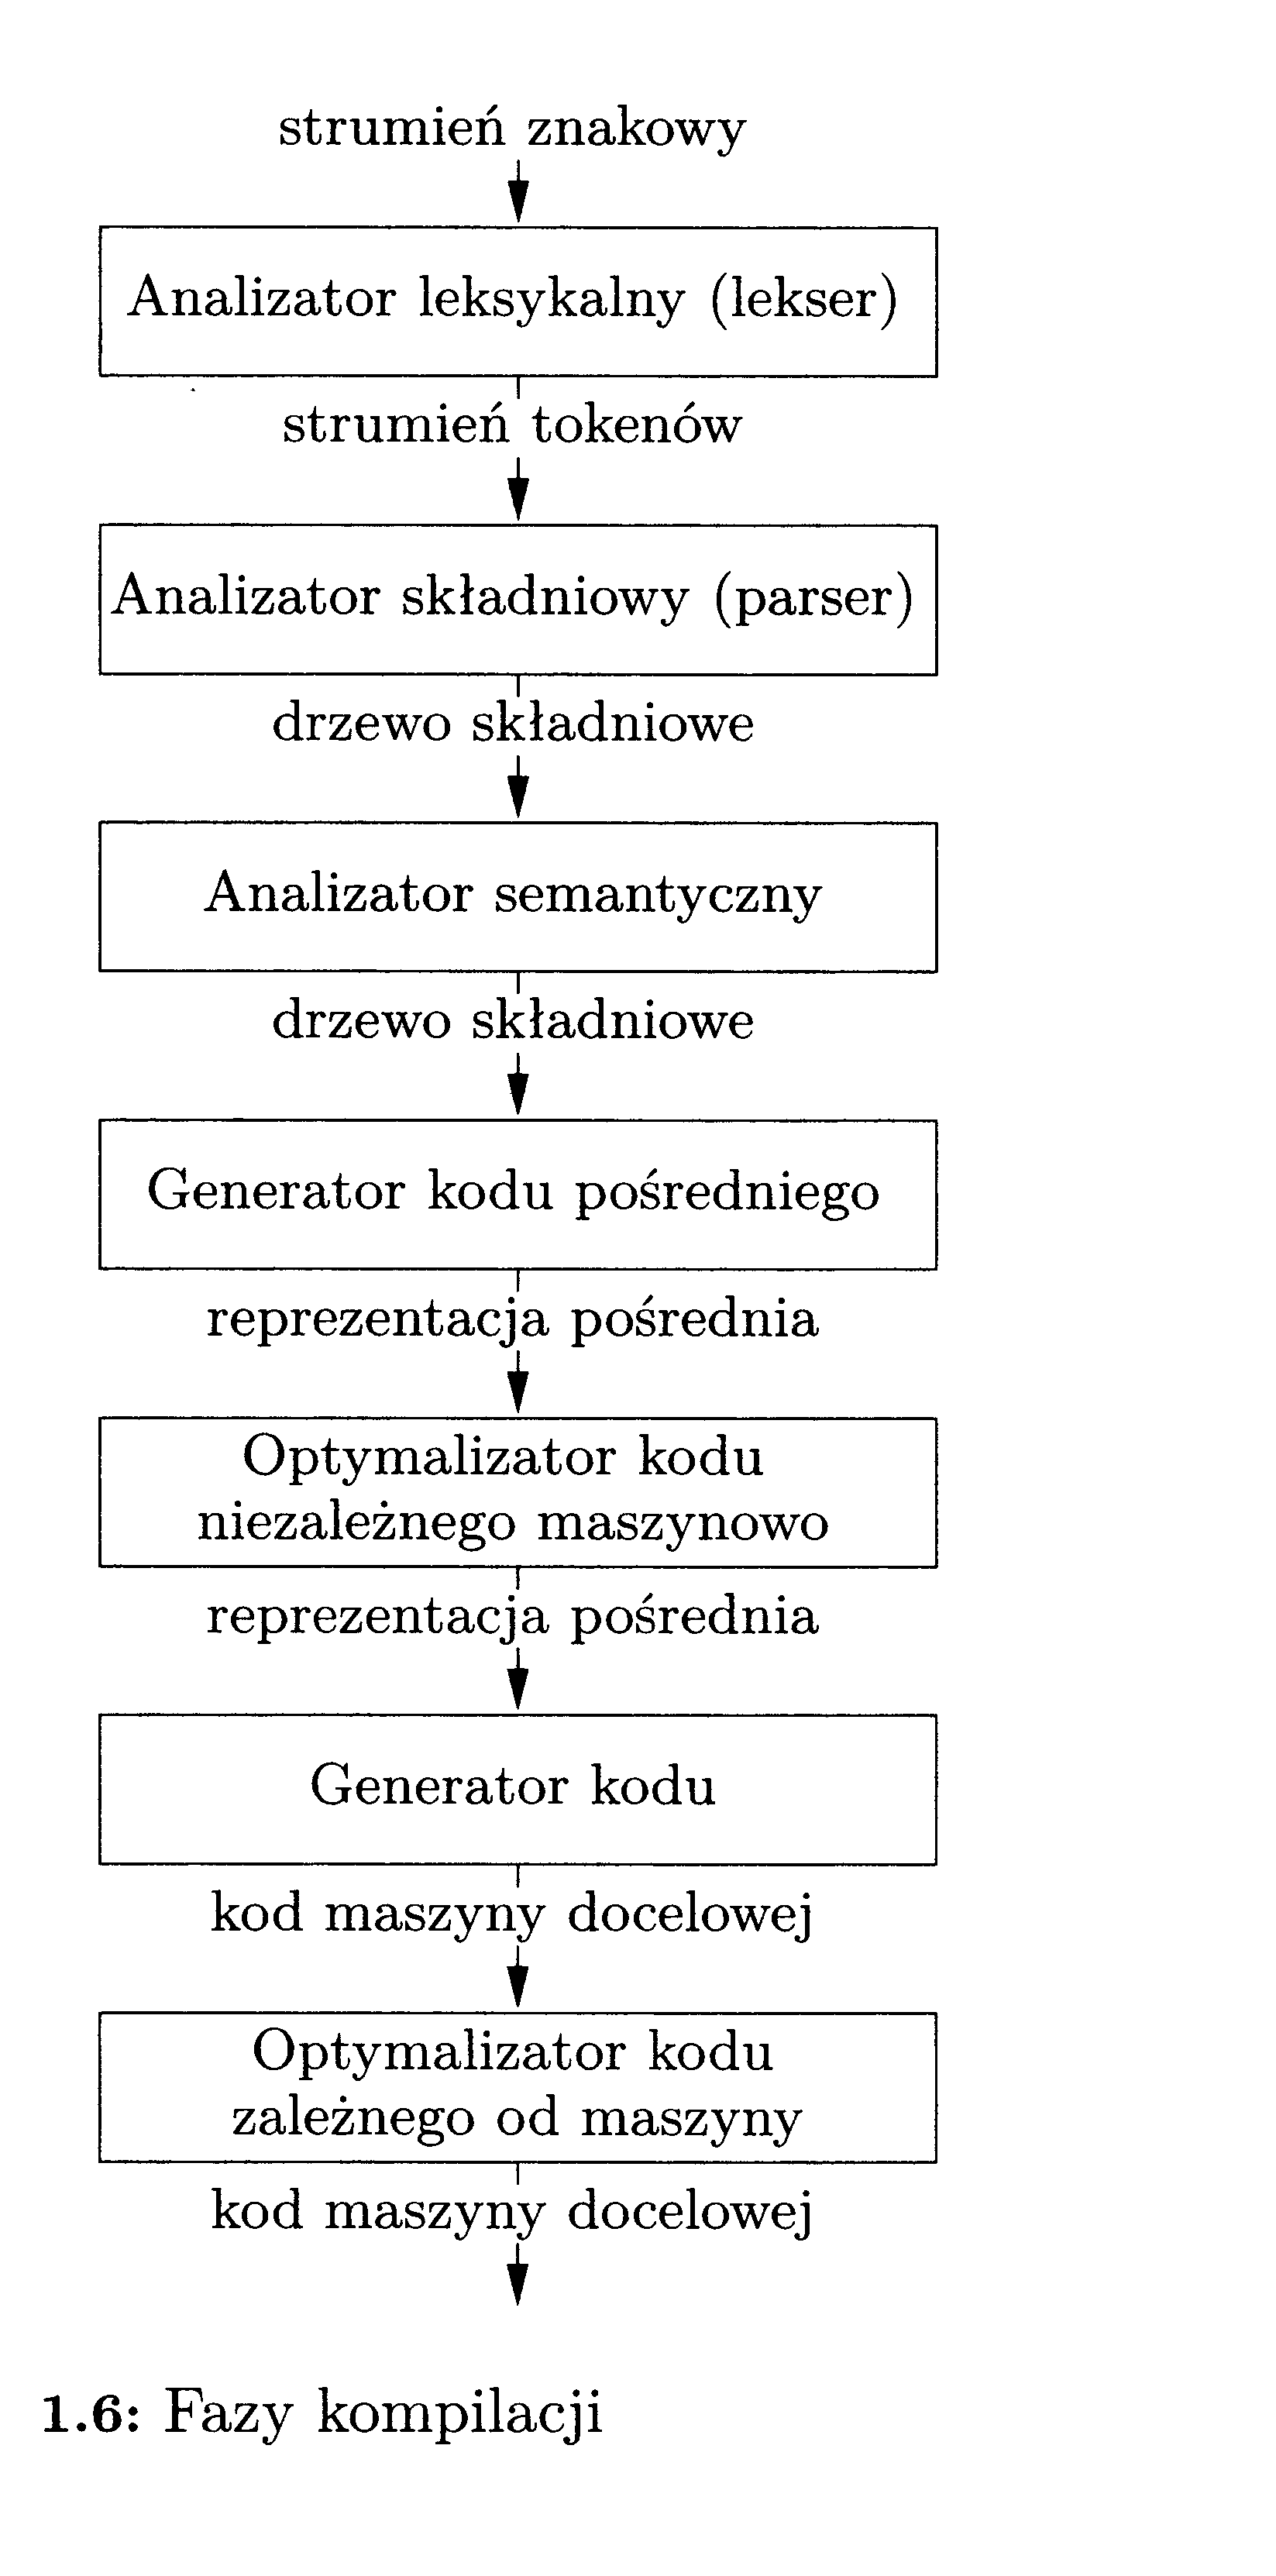
\includegraphics[height=0.8\linewidth]{images/wstep/fazy_kompilacji.png_bin_popr.png}
    \caption{Fazy kompilacji, zaczerpnięte ze str. 4 podręcznika\cite{DRAGON_BOOK}.}
\end{figure}

%\marginnote{W ostatnim bloku na rysunku powyżej powinien być optymalizator kodu zależnego od maszyny}
% W książce jest przeoczenie (pewnie tłumacza). Obrazek poprawiłem, mam to jakoś zaznaczyć?
 
Automatyczny translator musi rozłożyć zdanie w języku wejściowym, „zrozumieć” je, czyli przekształcić na wygodną dla niego reprezentację, aby z owego modelu złożyć reprezentację w języku docelowym. Wychodzi się od jednego napisu, dokonuje jego rozbioru, analizy, przeprowadza pewne operacje i sprawdzenia na odpowiednio skonstruowanych reprezentacjach głębszych konceptów wyrażanych za pomocą języka i potem „zwija” się je z powrotem do tekstu, tym razem w języku docelowym. Część analityczną nazywa się „front endem” , a syntetyczną „back endem”\cite[str.~4]{DRAGON_BOOK}.

Z dobrych powodów, sprowadzających się do zapewnienia porządku i możności rozumienia przez programistę, cały proces podzielony jest na fazy, odzwierciedlające się w warstwowej strukturze aplikacji tak, że można wizualizować kompilator jak na powyższym rysunku – jako łańcuch spiętych ze sobą komponentów przekazujących sobie kolejno przekształcane formy programu. Ma to pewne odniesienie do człowieka – my również prawdopodobnie posiadamy obwody w mózgu wyspecjalizowane w rozpoznawaniu znaków, liter i wyodrębnianiu z nich słów, przekazując sygnały do obwodów wyższego poziomu, układających słowa w sensy i zdania, a równocześnie odbywa się sięganie do pamięci, by przywołać znaczenia poszczególnych leksemów. Podobnie w kompilatorze analizator leksykalny zasila analizator składniowy (parser) i pisze się do tablicy symboli.

Niezależnie od tego, jak w rzeczywistości umysły ludzkie rozkładają zdania w językach naturalnych, lingwiści przywykli rozrysowywać strukturę zdań w postaci drzew składniowych (z podmiotem, orzeczeniem, przydawkami i innymi częściami zdania). Niektórzy z nich, zamiast gramatyk opisowych, w połowie XX w. w rozwinęli pojęcie „gramatyki generatywnej”, będącej zbiorem produkcji, ściśle określającej, jakie wyprowadzenia zdań są dozwolone\cite{Chomsky1956}. Podejście to, choć okazało się niewystarczające dla języków naturalnych, zaadoptowano, gdy zaczęto tworzyć sztuczne naśladownictwa naturalnych języków, zawężone i sformalizowane, a przez to możliwe do automatycznego tłumaczenia, w szczególności na kod maszynowy. 

%nagłówek tutaj jakiś
Zagadnienia analizy składniowej,  cytując Niklausa Wirtha, twórcę Pascala, „stanowią jedynie część problemów translacji i to w gruncie rzeczy stosunkowo niewielką. Jest to również część dająca się najłatwiej sformalizować, co m.in. pozwala na reprezentację składni języka w postaci dość regularnej struktury danych. Znacznie większe trudności napotykamy przy próbie formalizacji semantyki języka […]” \cite[str.~317]{wirth_alogorytmy_struktury_danych}.

O ile do dwóch pierwszych etapów rozwinięto ścisłą, użyteczną i dość uniwersalną teorię\cite{martin1998intuitionistic_types, TAPL}, o tyle nie wypracowano tak rozbudowanego aparatu analizy semantycznej w innych aspektach niż systemy typów, nie jest ona szeroko opisywana i programista kompilatora polegać musi w wielkiej części na własnej inwencji\cite{waite_goos}. Dzieje się tak dlatego, że owa środkowa część kompilatora najbardziej odpowiada idiosynkrazjom konkretnego języka. W tym etapie, przekształcamy program od drzewa rozbioru, zależnego prawie wyłącznie od formalizmu gramatyki, do pośredniej postaci, bliższej maszynie, przydatnej przy optymalizacjach, rządzonych równie potężnymi formalizmami matematycznymi. 

Znajdująca się pomiędzy tymi dwoma terytoriami, poddanymi ścisłym badaniom, warstwa pośrednia przetwarza najbardziej analityczną postać programu, gdzie wszystkie jego językowe własności zostają rozkodowane z tekstu źródłowego i przechowywane jawnie w strukturach danych, odpowiadających bezpośrednio konceptom języka. Tam zakres leksykalny reprezentowany jest określoną strukturą zawierającą listę symboli, typ danej zmiennej jest osobnym  obiektem, klasa przechowywania (static/automatic z C) pewną wartością wyliczeniową. Niechybnie musi zatem ta faza charakteryzować się wielką zmiennością, w zależności od języka – translator języka obiektowego będzie zawierał reprezentację klasy i będzie ona wręcz centralna dla modelu danych. W funkcyjnym języku przeciwnie, reprezentacje funkcji, ich typów i domknięć zajmą poczesne miejsce. Zakodować też musimy tam wszystkie drobne szczegóły i reguły semantyczne jakie język posiada. Dlatego obok coraz potężniejszych teorii typów, oraz przydatnych raczej na początku tej fazy gramatyk atrybutywnych, nie istnieje ogólnie przyjęta teoria, ani nawet praktyczny przepis na realizację analizy semantycznej.

Inaczej ma się rzecz z optymalizacjami. Nie można ich pominąć – to, że pierwszy kompilator Fortranu (jednocześnie pierwszy w historii kompilator języka wysokiego poziomu), w ogóle został przyjęty przez środowisko informatyczne, umożliwiło zapewnienie, że tworzy kod maszynowy prawie zawsze tak samo szybki, jak programista asemblerowy. Największą zaletą w oczach współczesnych mogła nawet nie być możliwość prawie dosłownego przepisywania wyrażeń matematycznych, a efektywne rozplanowywanie wielokrotnych pętli przy operacjach macierzowych (na tablicach z wieloma indeksami), która to czynność zajmowała wcześniej programistom ogromne ilości czasu i była podatna na błędy, nie chciano jednak godzić się na żadne interpretery, czy prymitywne rozwiązania, drżąc przed roztrwonieniem przez nie wątłych zasobów ówczesnych komputerów\cite{FORTRAN_AUTOMATIC_CODING_SYSTEM}.
Odnoszę się do tych zamierzchłych dyskusji, aby uzmysłowić, jak centralnym zagadnieniem kompilacji są optymalizacje i bez nich, bez produkcji równie efektywnego kodu, jak byłoby to możliwe ręcznie w języku docelowym, nie można mówić o prawdziwie użytecznym  kompilatorze.
%<też do przepisania>

Problemy analizy przepływu, przenoszenia niezmiennego kodu na zewnątrz pętli, detekcji kodu martwego, efektywnego traktowania rekursji ogonowej i niemożliwe do wymienienia tutaj rzesze optymalizacji wynalezionych na przestrzeni ostatnich dziesięcioleci, są naturalnie trudne, zaryzykuję stwierdzenie, że wielokroć trudniejsze od parsingu, bo wymagają bardzo ścisłej wiedzy matematycznej, nie są też tak często przedmiotem kursów na uczelniach. I te zagadnienia mogą się wydać relatywnie zachęcające, gdyż dalej w procesie translacji schodzić trzeba w głąb, aż do fizycznej maszyny – problem przydziału rejestrów nie dość, że jest NP-zupełny\cite{REGISTER_ALLOCATION_CHAITIN1981, REGISTER_ALLOCATION_2}, to jeszcze zależny od konkretnych technikaliów maszyny cyfrowej. W niektórych architekturach pewne rejestry mogą mieć szczególne ograniczenia, poszczególne instrukcje właściwe tylko sobie zachowania. Na przykład, na znanej nam wszystkim 32 bitowej architekturze Intela, dwa operatory całkowite znane z C – dzielenia i modulo (/ i \%) tłumaczone są na tę samą instrukcję, IDIV bowiem pozostawia ona iloraz w rejestrze eax a resztę w edx – o wszystkich takich szczegółach należy pamiętać i uwzględnić w algorytmach. Podczas generacji kodu trzeba również, oprócz realizacji oczywistych schematów translacji dla warunków i pętli, generować tablice skoków dla switch, przy wywołaniach budować ramki stosu i zapisywać niektóre rejestry, zależnie od architektury i konwencji, a jeśli umieściło się w języku wyjątki podobne tym z C++, należy wygenerować zupełnie nietrywialny kod do ich obsługi. W całości składa się to na niezwykle pracochłonne zadanie, które wszak należy powtórzyć, prawie zupełnie niezależnie dla każdej architektury docelowej.

Nie jest to wszak koniec procesu translacji, nie ostatni komponent na rycinie zamieszczonej powyżej – mając nawet wygenerowany wykonywalny kod obiektowy, nie możemy załadować go verbatim do pamięci maszyny, ustawić na konsoli operatora wartości licznika rozkazów i nacisnąć guzika – jak ongiś się zdarzało – kod trzeba jeszcze skonsolidować i przygotować do interakcji z programem ładującym systemu operacyjnego, aby mógł on przekształcić nasz obraz binarny w „żywy” obraz procesu. Jeśli ktoś sądzi, że jest to jedynie kwestia przekazywania odpowiednich flag do GNU ld (albo odpowiednika w danych systemie operacyjnym), niech przeczyta poniższy wycinek i policzy ile zna osób wiedzących czym jest skrypt linkera, a co dopiero potrafiących takowy zrozumieć i ocenić poprawność.
(Poniżej fragment domyślnego skryptu ld dla formatu ELF na architekturze x86-64, przedrukowany za \cite{default_ld_linker_script}.)

\begin{lstlisting}[
    basicstyle=\footnotesize, %or \small or \footnotesize etc.
]
.plt            : { *(.plt) *(.iplt) }
.plt.got        : { *(.plt.got) }
.plt.bnd        : { *(.plt.bnd) }
  .text           :
  {
    *(.text.unlikely .text.*_unlikely .text.unlikely.*)
    *(.text.exit .text.exit.*)
    *(.text.startup .text.startup.*)
    *(.text.hot .text.hot.*)
    *(.text .stub .text.* .gnu.linkonce.t.*)
    /* .gnu.warning sections are handled specially by elf32.em.  */
    *(.gnu.warning)
  }
  .fini           :
  {
    KEEP (*(SORT_NONE(.fini)))
  }
  PROVIDE (__etext = .);
  PROVIDE (_etext = .);
  PROVIDE (etext = .);
  .rodata         : { *(.rodata .rodata.* .gnu.linkonce.r.*) }
  .rodata1        : { *(.rodata1) }
  .eh_frame_hdr : { *(.eh_frame_hdr) *(.eh_frame_entry .eh_frame_entry.*) }
  .eh_frame       : ONLY_IF_RO { KEEP (*(.eh_frame)) *(.eh_frame.*) }
  .gcc_except_table   : ONLY_IF_RO { *(.gcc_except_table
  .gcc_except_table.*) }
  .gnu_extab   : ONLY_IF_RO { *(.gnu_extab*) }
  /* These sections are generated by the Sun/Oracle C++ compiler.  */
  .exception_ranges   : ONLY_IF_RO { *(.exception_ranges
  .exception_ranges*) }
  /* Adjust the address for the data segment.  We want to adjust up to
     the same address within the page on the next page up.  */
  . = DATA_SEGMENT_ALIGN (CONSTANT (MAXPAGESIZE), CONSTANT (COMMONPAGESIZE));
  /* Exception handling  */
  .eh_frame       : ONLY_IF_RW { KEEP (*(.eh_frame)) *(.eh_frame.*) }
  .gnu_extab      : ONLY_IF_RW { *(.gnu_extab) }
  .gcc_except_table   : ONLY_IF_RW { *(.gcc_except_table .gcc_except_table.*) }
  .exception_ranges   : ONLY_IF_RW { *(.exception_ranges .exception_ranges*) }
  /* Thread Local Storage sections  */
  .tdata	  : { *(.tdata .tdata.* .gnu.linkonce.td.*) }
  .tbss		  : { *(.tbss .tbss.* .gnu.linkonce.tb.*) *(.tcommon) }
\end{lstlisting}

Potrzebę rozumienia uwydatniają komentarze do osobnych sekcji, które kompilatory C++ generować muszą specjalnie po to, by zapewnic działanie mechanizm wyjątków (np. .gnu\_extab), czy statycznej inicjalizacji w tym języku (.init/.fini/.ctors/.init\_array). To drugie pokazuje, że nawet tak głęboko ukryte szczegóły implementacyjne mają wpływ na język programowania na najwyższym poziomie – bo sposób działania konsolidatora (linkera) i przetwarzania przez niego tych specjalnych sekcji powoduje w C++ realne i kłopotliwe zjawisko zjawisko zwane „Static initialization order fiasco”\cite{siof}. (Nie da się wymusić deterministycznego porządku wykonywania statycznych inicjalizatorów znajdujących się w różnych plikach), które skutkuje tym, że obecnie odradza się stosowanie tego mechanizmu w ogóle\cite{google_cpp_guidelines_static}.

\section{Historyczne oszacowania kosztów wytwarzania kompilatorów}
Pozwoliłem sobie na ów korowód szczegółów, aby umotywować, dlaczego tak wiele języków odeszło od generowania kodu dla fizycznych maszyn, na rzecz używania maszyn wirtualnych, albo w ogóle intepreterów – pozwala to relatywnie zmniejszyć złożoność problemów generacji kodu i osiągnąć większą przenośność, jeśli maszyna wirtualna jest pisana np. w C, którego kompilatory istnieją na chyba wszystkich powszechnych architekturach.

Prócz tego chciałem pokazać, jak rozległym tematem jest kompilacja i że w klasycznym ujęciu, obejmującym wszystkie wymienione fazy, znajduje się poza zasięgiem jednego człowieka, a tworzenie praktycznie użytecznych języków w celu badania ich własności, zadaniem niewykonalnym. Dość powiedzieć, że wedle raportu projektowego, napisanie wspomnianego już pierwszego kompilatora Fortranu, po fakcie wyceniono na 18 roboczolat (!), rozłożonych na kilku programistów w ciągu dwóch i pół roku\cite{FORTRAN_AUTOMATIC_CODING_SYSTEM}.

Niklaus Wirth, również wspomina tworzenie kompilatora Pascala, jako grupowe, wielomiesięczne przedsięwzięcie, prowadzone do tego technikami, zapewne niedostępnymi ordynarnym programistom. (Po zaprojektowaniu języka Pascal, napisano jego pierwszy kompilator w nim samym i przetłumaczono go ręcznie na asembler komputera IBM 704)\cite{Wirth_recollections_Pascal}. Spoglądając w bardziej współczesne czasy, można ocenić tytaniczny wysiłek włożony w gcc, g++, czy inne kompilatory (ostatnio wystarczy spojrzeć na repozytorium projektu), by zwątpić, czy językotwórstwo badawcze, eksploracyjne, czy podyktowane zwyczajnie własnymi upodobaniami ma szansę w ogóle się ziścić.
%wspomniec o prototypie????

% Każdy z tych etapów stawał się z czasem coraz bardziej złożony:
% gramatyki zwiększały rozmiar, wzrast ze wzrostem poziomu abstrakcji, więc i parsery stawały się coraz bardziej skomplikowane i trudne do napisania, podnosił się też poziom wymagań względem komunikatów o błędach,
% reprezentacje wewnętrznych obiektów musiały stawać się coraz bardziej skomplikowane, zarówno z powodu wzrostu poziomu abstrakcji (potrzeby modelowania np. klas oprócz funkcji, typów generycznych prócz prostych), jak polepszenia optymalizacji, same optymalizacje stały coraz doskonalsze 

%[https://www.researchgate.net/figure/The-large-scale-evolution-of-programming-languages-1953-2012-Lineages-of-influence_fig1_305418676]


\section{Jak zmniejszyć koszt wytworzenia kompilatora?}
Jak w wielu dziedzinach informatyki – wykorzystując odpowiednie narzędzia. Kilkadziesiąt lat intensywnego rozwoju teorii kompilacji naturalnie nie przyniosło jedynie rozrostu tematu, lecz i próby jego syntez i automatyzacji podzagadnień w postaci programów i bibliotek. Przytoczmy jeszcze raz diagram faz translacji, zaznaczając na nim tym razem to, co można uprościć z użyciem narzędzi.
\begin{figure}[H]
    \centering
    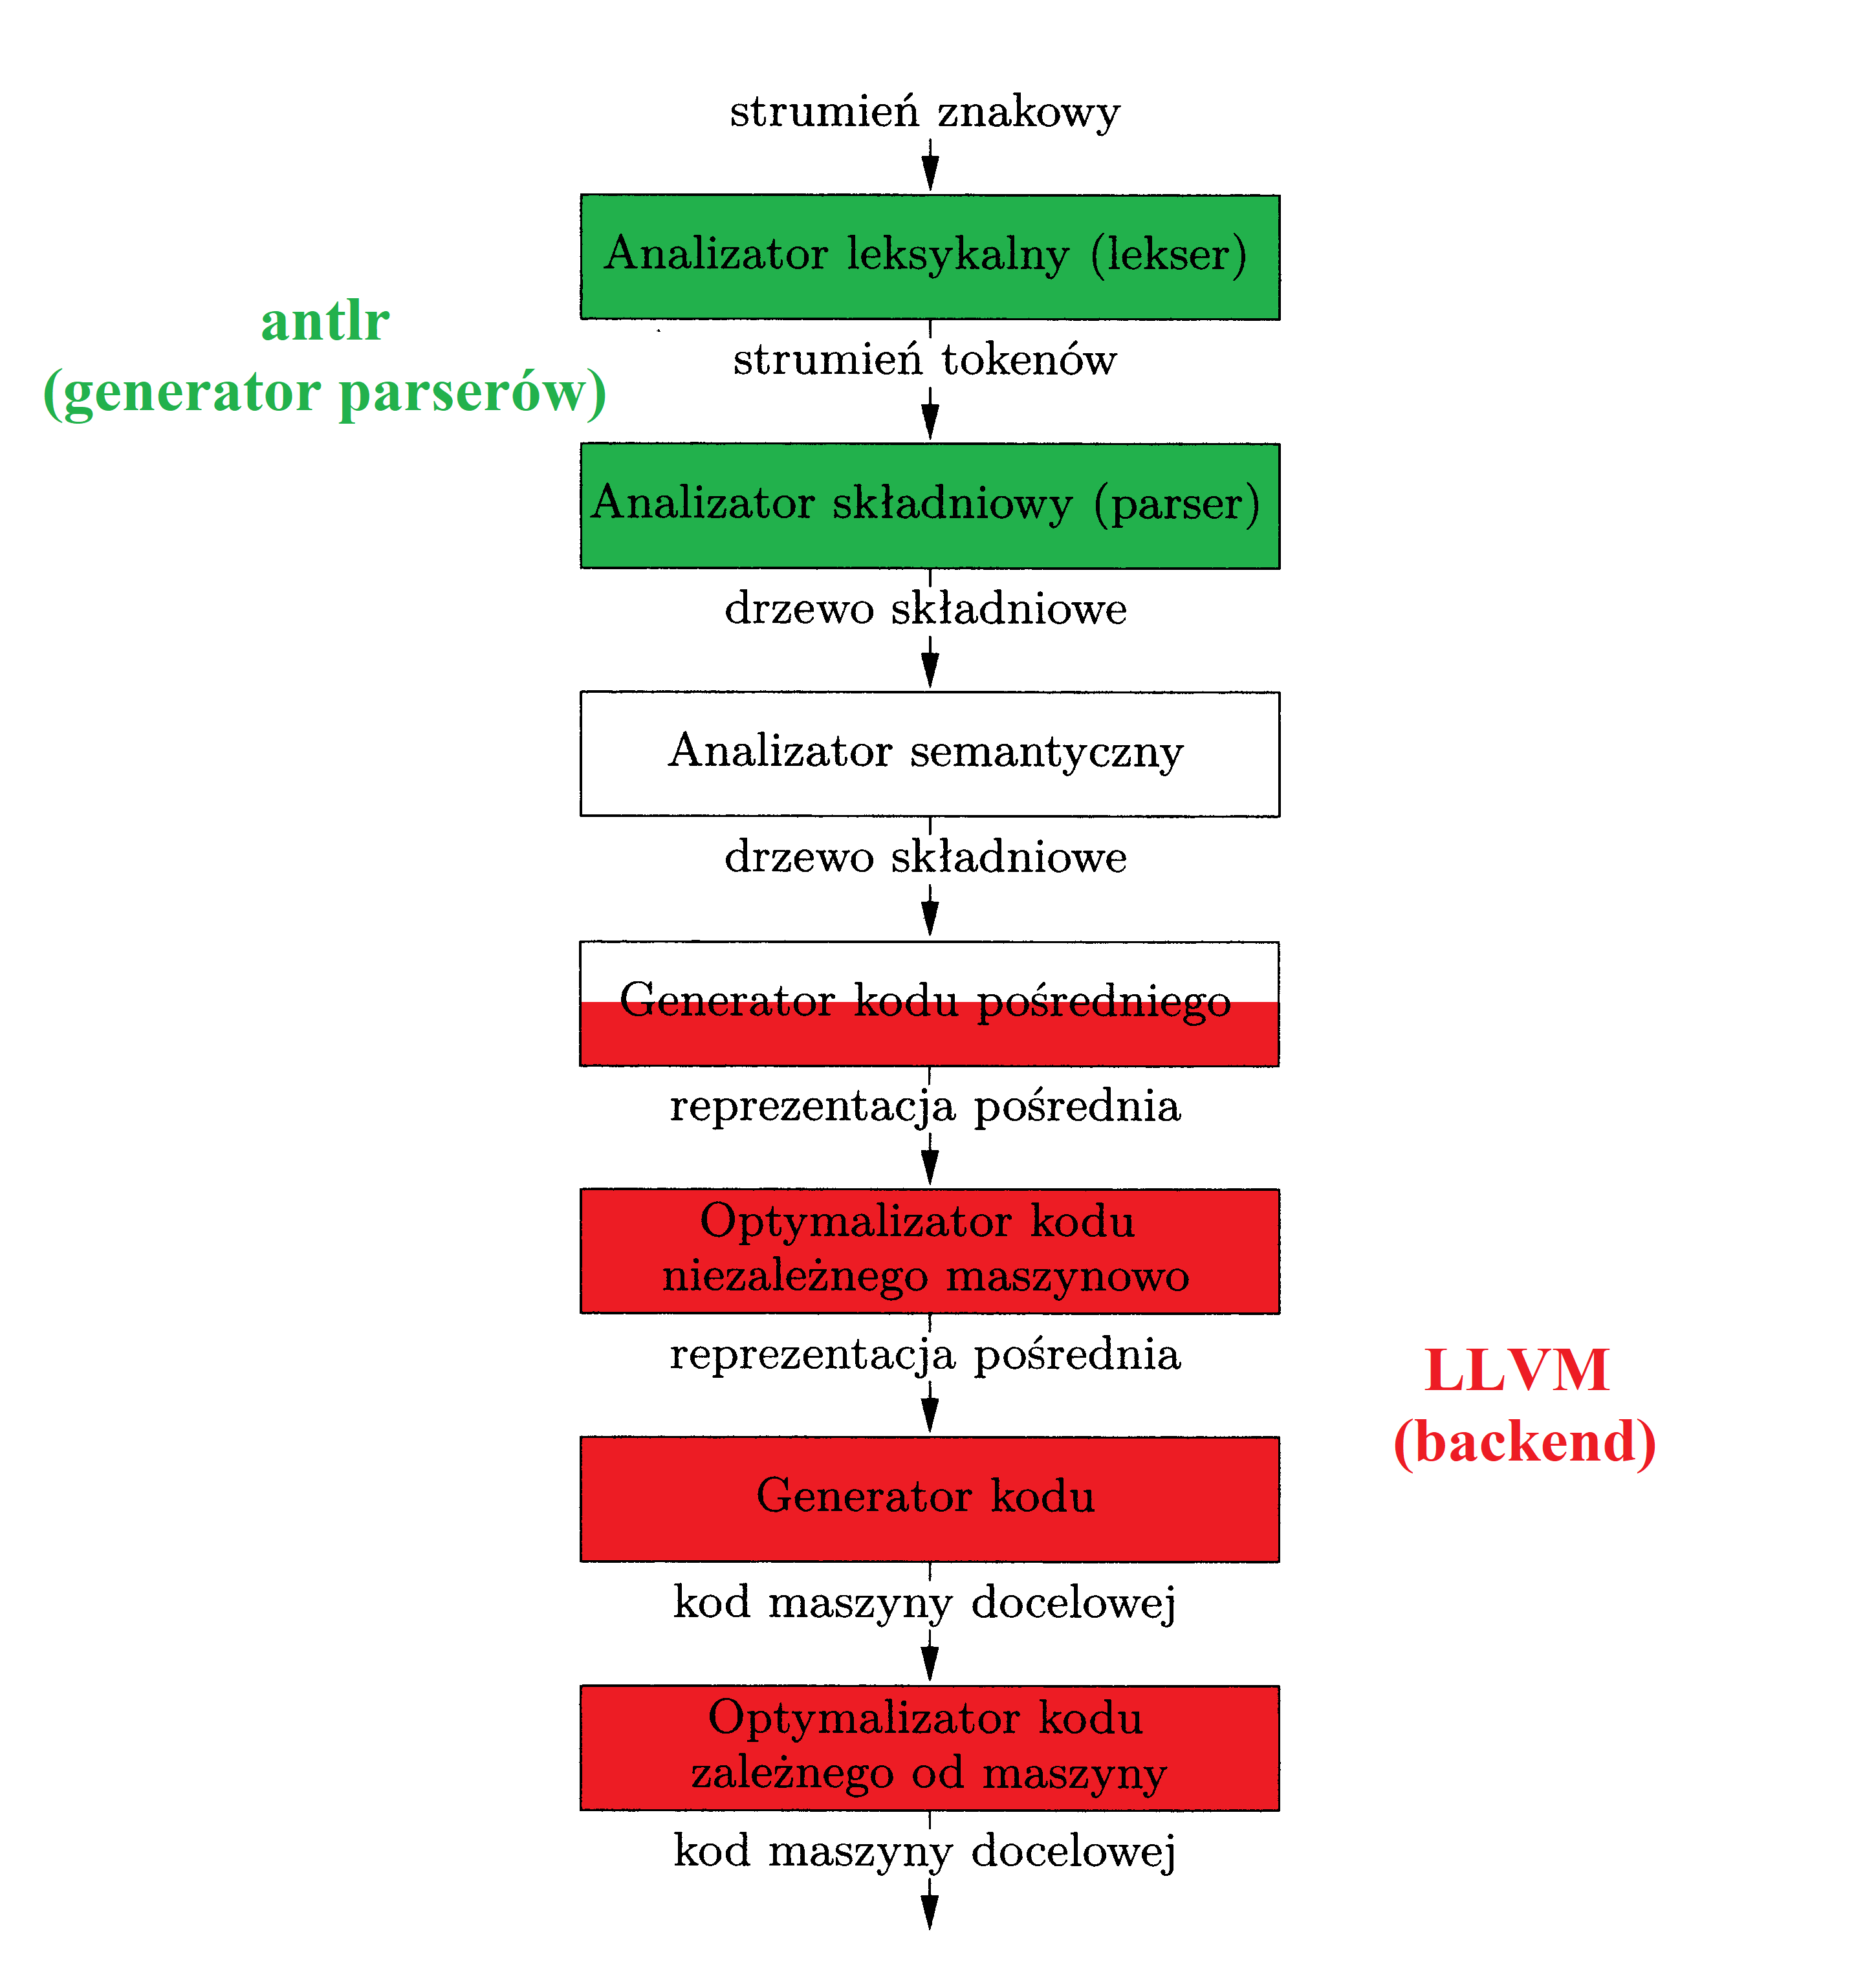
\includegraphics[height=0.8\linewidth]{images/wstep/fazy_kompilacji.png_bin_antlr_llvm_podpisany_popr.png}
    \caption{Fazy kompilacji, zaczerpnięte ze str. 4 podręcznika\cite{DRAGON_BOOK}, z zaznaczonym pokryciem przez narzędzia}
\end{figure}

%\marginnote{W ostatnim bloku na rysunku powyżej powinien być optymalizator kodu zależnego od maszyny}
% Jak w poprzednim  - poprawiłem na obrazku, mam to jakoś zaznaczyć w podpisie?

Uzyskawszy teorię języków formalnych, gdzie niemal kompletnym opisem składni języka jest jego gramatyka, często w jednolitej notacji Backusa-Naura, nie trzeba było długo czekać, aż podjęto próby automatyzacji procesu tworzenia parserów. Para uniksowych programów z lat siedemdziesiątych – lex i yacc (yet another compiler compiler) ma niebagatelny wpływ na historię informatyki, z ich użyciem stworzono nie tylko tak proste języki jak awk, lecz tak złożone jak perl\cite{parsing_timeline_kegler}, a do 2006 roku gcc używało ich do tłumaczenia C\cite{gcc_2006_release_note}.
%(*właściwie to ulepszonych wersji – flex i bison). 

Programy tego typu przyjmują jako plik wejściowy gramatykę języka w formacie będącym zazwyczaj ich autorskim rozszerzeniem notacji EBNF, zezwalającym często na umieszczanie wewnątrz produkcji gramatycznych bezpośrednio fragmentów kodu i generują parser. Oprócz lexa i yacca obecnie istnieje tak dużo wartych uwagi rozwiązań, że wybór najlepszej opcji może okazać się trudny, zwłaszcza jeśli nie ma się jeszcze doświadczenia w temacie. W rozdziale \ref{cha:wywodJezyka} opisane zostaną nieco dokładniej techniki parsingu i umotywowany zostanie wybór konkretnego generatora parserów. W tym miejscu wystarczy nam wiedza, że dla względnie niewielkich języków, podlegających częstym zmianom i rozwojowi, generowany parser oszczędza wiele pracy – o wiele łatwiej jest zmienić gramatykę języka, niż przepisać (być może znaczną) część procedur ręcznie pisanego parsera rekursywnie schodzącego. Wprawdzie dla wielkich języków programowania parsery ręcznie napisane okazują się mieć w ostatnich latach znaczną popularność, szczególnie dlatego, że można w nich dokonywać wedle woli subtelnych zmian ulepszających komunikaty o błędach.
%[https://notes.eatonphil.com/parser-generators-vs-handwritten-parsers-survey-2021.html]
%[https://www.quora.com/What-is-a-good-parser-generator-for-a-project-Is-YACC-the-best-considering-speed-as-a-factor-too]
%[https://lukasatkinson.de/2015/marpa-overview/ - śmieszne]%może do opisu parsingu
%[https://rahul.gopinath.org/post/2021/02/06/earley-parsing/]

Znaleźliśmy zatem narzędzia skracające znacząco czas pisania „przedniej” części kompilatora, „środkowa”, jak już powiedzieliśmy bardzo silnie zależy od tłumaczonego języka, więc nie jest przyjaznym środowiskiem dla ogólnych narzędzi, pozostaje jeszcze „tylna” – optymalizacje i generowanie kodu wynikowego. Wracamy w ten sposób do zapowiedzianego LLVM. 

%{clang i LLVM}
Kompilator clang stworzono, przepisując na nowo gcc, po części z powodów licencyjnych (ze strony Apple pierwotnie finansującego przedsięwzięcie), po części chcąc zastosować nowsze techniki, które nie miałyby miejsca w kodzie programu tak dojrzałego i mającego kluczowe znaczenia dla naszej cywilizacji (nie jest to przesada, skoro kompiluje się przy pomocy gcc w zasadzie ,,wszystko'', z jądrem Linuksa włącznie). Oddano przy tym światu dodatkowo wielką przysługę. Warstwowość architektury kompilatora, jak powiedzieliśmy, wynika naturalnie z zasad jego funkcjonowania, a pewna modularność kodu jest koniecznością w tak wielkim projekcie i uznaną obecnie dobrą praktyką programistyczną, w tym jednak wypadku, oprócz wydzielenia back-endu, zdecydowano się wyeksponować go jako osobny projekt - LLVM, definiując publicznie dostępny interfejs programistyczny (API), wraz z językiem pośrednim z którego korzysta zarówno kompilator C, jak i C++. Dość szybko zauważono, że można stworzyć własny „front-end” dla dowolnego języka, dającego się tłumaczyć do postaci pośredniej LLVM (LLVM IR), w dodatku otrzymuje się wtedy zupełnie „za darmo” całe nieprzebrane bogactwo optymalizacji potężnych, wymagających zastosowania wysokiej matematyki, bądź zwyczajnie żmudnych w implementacji – wszystkich, które zespół clanga musiał odtworzyć, by choć marzyć o doścignięciu wydajności kodu wynikowego gcc (i późniejszego prześcignięcia). W dodatku zyskujemy możliwość generacji kodu na tyle architektur, na ile portowano clanga, nie jest to liczba tak wielka, jak tych, dla których jakikolwiek kompilator C jest dostępny, jednak i tak przekracza ilość, która uzyskałby nawet duży kompilator pisany od początku do końca. W najbardziej praktycznym sensie, otrzymujemy ,,za darmo'' wsparcie dla popularnych architektur, których użytkownikami jesteśmy, albo spotykamy się najczęściej – IA-32, (potocznie x68), IA-64 (potocznie x86-64) i rozmaite wersje ARM.\cite{llvm_org, forum_llvm_apple_licenses}
%[https://forums.freebsd.org/threads/apple-originally-tried-to-give-gpled-llvm-to-gcc.44533/ i linki poniżej]

Reprezentacja pośrednia (LLVM IR), a raczej struktury danych i wywołania, które należy użyć, aby zacząć wykorzystywać programowo jej potencjał, nie należą wprawdzie do najbardziej oczywistych, lecz są w zasięgu pojedynczego programisty, co pokazują rozmaite materiały dostępne w sieci\cite{kalleidoscope}, jak i zostanie zademonstrowane na praktycznych przykładach w dalszej części pracy.

\section{Dlaczego nie użyć maszyny wirtualnej?}
Nawet po przedstawieniu zalet LLVM, takie pytanie wciąż może niepokoić czytelnika, mając na uwadze, że użycie LLVM wymaga wiedzy niskopoziomowej, podczas gdy pisząc własną maszynę wirtualną, można niemal skutecznie odgrodzić się od sprzętu i skupić się jedynie na bardziej abstrakcyjnych zagadnieniach językowych. 
Odpowiedzią przewrotną na to pytanie jest, że przecież korzystamy z maszyny wirtualnej – LLVM to wszak „Low-Level Virtual Machine”, jedną z jego możliwości jest wygenerowanie statycznego kodu maszynowego, posiada jednak również moduł JIT (just-in-time), reprezentujący tę samą zasadę działania co w roku 2024 najpopularniejsza implementacja Pythona - cpython. (zob. katalogi \_\_pycache\_\_ i pliki .pyc wewnątrz). Żeby odpowiednio rozwikłać te wątpliwość, zbierzmy w tym miejscy wymagania projektowe.

\textbf{Wymagania projektowe względem programu translatora}
\begin{itemize}[noitemsep]
    \item Architektonicznie przystosowany do częstych modyfikacji języka i eksperymentów.%Dla niedużego, łatwo modyfikowalnego (w celu eksperymentów) języka. -- lepiej?
    \item Niewielki, zdatny do napisania i przetestowania przez jedną osobę w ciągu kilku miesięcy.
\end{itemize}
%\marginnote{Powyżej są dwa osobne punkty ((item) czy jeden?}
%Miały być dwa...

Nie jest to długa lista, choć oszacowanie kosztów może wydać się nazbyt optymistyczne, w świetle podanych wcześniej liczb (18 roboczolat dla pierwszego Fortranu), to współczesne narzędzia, jak i ogólny rozwój technik programistycznych, możliwości sprzętowych, czynią redukcję takich rozmiarów na wyciągniecie ręki Nie obieram też za cel stworzenia translatora, jak tamten, zmieniającego postać informatyki, czy „zaledwie” powszechnych praktyk programistycznych, ani nawet stworzenia nowego popularnego języka, mam na uwadze jedynie praktyczne i pouczające ćwiczenie w zakresie projektowania języków programowania.

Paradoksalnie ze względu na takie ograniczenia dostępnych zasobów, uważam tworzenie własnej maszyny wirtualnej za gorszą decyzję, o ile tłumaczy się język imperatywny (a wybieram go ze względu na prostotę i niewielką sumę własnych doświadczeń np. z językami funkcyjnymi) Wystarczy uważnie spojrzeć w obecny kod źródłowy cpythona, w główną pętlę jego maszyny wirtualnej\cite{cpython_main_loop}, by pojąć, że napisanie własnej jest również wyzwaniem, wymagającym szczególnej wiedzy, o charakterze być może porównywalnym do tej, koniecznej do pracy z abstrakcjami rzeczywistego sprzętu pokroju LLVM. Najważniejszym czynnikiem dla mnie było wszak oszacowanie kosztu doprowadzenia własnej maszyny wirtualnej do wymaganej niezawodności. Wszelkie pomyłki w niej popełnione wpływałyby na zachowanie całego systemu, zaciemniając problemy w innych częściach translatora i utrudniając ich analizę. 

%%ograniczenie lokalizacji błędów
Używając zarówno generatora parserów, jak i gotowego back-endu, niemal cały wysiłek ściśle programistyczny skupia się w relatywnie niewielkiej środkowej fazie, co zapewnia tak pożądaną redukcję problemu i zlokalizowanie go w jednym podsystemie o dobrze określonych granicach. Błędy prozaicznej natury w pozostałych fazach translacji można niemal wykluczyć, ponieważ wykorzystane narzędzia są intensywnie i profesjonalnie testowane. Występujące problemy można niemal od razu ograniczyć do środkowej fazy, defekty gramatyki objawiają się w odmienny sposób, a niewłaściwe użycie LLVM karane jest zazwyczaj surowo, acz rozpoznawalnie. 

Dodatkowym istotnym czynnikiem, wpływającym na wybór statycznie kompilowanego kodu maszynowego jest kwestia biblioteki standardowej. Praktyka programistyczna sugeruje, że o przydatności języka programowania i subiektywnej ocenie doświadczeń z nim związanych decyduje nie tylko jego składnia, system typów, czy nawet przyjazny edytor (czy dziś raczej IDE), ale w wielkiej części zbiór łatwo dostępnych funkcji (czy procedur) – biblioteka standardowa, ewentualnie możliwość łatwego, powtarzalnego instalowania bibliotek i zarządzania ich zależnościami.

Systemy pakietów, choć pojawiają się powszechnie w nowych językach, nawet tak niskopoziomowych jak Rust, wiążą się jednak z dodatkowym, znacznym wysiłkiem programistycznym, potrzebnym by w ogóle móc zacząć przydatne pakiety pisać. Nie sądzę, by napisanie praktycznie użytecznej biblioteki standardowej było w zasięgu projektu tego rozmiaru, mając na uwadze, jak wiele pracy włożono w biblioteki standardowe C, C++, czy w powszechnie używane w Pythonie pakiety. Intrygującym pytaniem jawi się systematyczne porównanie ilości pracy włożonej w kompilator danego języka i w jego bibliotekę standardową rozszerzoną o popularne biblioteki.

Z tego powodu, za najrozsądniejsze rozwiązanie dla prostego, imperatywnego języka uważam skorzystanie z libc, a LLVM zapewnia nie tylko taką możliwość, lecz zgodność z binarnym interfejsem C (C ABI) w danym środowisku. Zatem w praktyce wszystko to, co można wywołać bądź użyć z C, jest potencjalnie dostępne również dla języka tłumaczonego z użyciem LLVM.

Pomimo ogromnych możliwości samego LLVM w zakresie generacji optymalnego kodu, ze względu na nadrzędne tu dążenie do redukcji zadania, w zakresie efektywności faktycznie generowanego kodu, przyjmijmy jedynie skromne wymaganie: „translator nie produkuje programów rażąco nieefektywnych”. Pozwoli to uchronić się przed wszelkimi zgubnymi formami przedwczesnej optymalizacji i mieć na uwadze charakter języka i docelową grupę jego użytkowników. Kompilatory wielkich języków ogólnego przeznaczenia tłumaczą zarówno kod aplikacji o krytycznym znaczeniu, gdzie ewentualny spadek wydajności w następnej wersji jest automatycznie monitorowany (np. postgres\cite{postgres_regression_testing}), jak i ogromne wielomegabajtowe źródła  wygenerowane przez transpilery czy domenowe narzędzia, poddające próbie wydajność samego procesu przekładu.

Trzeźwo określmy, że grupą docelową tego projektu będzie co najwyżej wąska grupa osób zainteresowanych, kody źródłowe nie będą wielomegabajtowej wielkości, szybkość działania programów nie będzie najważniejszą metryką. Podwaliny pod zoptymalizowany i szybki kod zapewnia LLVM i będzie można je w przyszłości wykorzystać. Możliwości zaś, uwolnione przez to obniżenie wymagań, zostaną spożytkowane w architekturze translatora, prowadząc do jego większej przejrzystości, utrzymywalności i ułatwionego śledzenia błędów.


\section{Podsumowanie wymagań}
Na koniec tego rozdziału zbierzmy w jednym miejscu określone wymagania i cel przedsięwzięcia.

\textbf{Wymagania względem języka:}
\begin{itemize}[noitemsep]
    \item prosty
    \item imperatywny
    \item relatywnie niskopoziomowy
    \item kompilowany
    \item statycznie typowany
\end{itemize}

\textbf{Wymagania projektowe, względem translatora:}
\begin{itemize}[noitemsep]
    \item Niewielki, zdatny do napisania przez jedną, dobrze zmotywowaną osobę w kilka miesięcy.
    \item Modularny, łatwy do debugowania
    \item Łatwy do modyfikacji wraz z rozwojem języka
    \item O niezawodności możliwie zbliżonej do standardu w dziedzinie.
\end{itemize}

\textbf{Wymagania techniczne:}
\begin{itemize}[noitemsep]
    \item Parser generowany wygodnym narzędziem.
    \item Statycznie kompilowany, używając LLVM jako „back-endu”.
\end{itemize}

\textbf{Wymagania pragmatyczne:}
\begin{itemize}[noitemsep]
    \item Wykorzystanie biblioteki standardowej C, potencjalnie innych, dostępnych przez C ABI.
    \item Translator nie produkuje programów „rażąco niefektywnych”
\end{itemize}